
\section{Bi-Directional Merging}

Although it is not a metric, we introduce the concept of a merging one
set with another.
To begin with, for a string \(w \in \Sigma^\star\)
and a set \(A \subseteq \Sigma^\star\).
The merging cost of \(x\) into \(A\) can be defined as:

\begin{align*}
  m_w \parens{x, A} = \inf_{a \in A} d\parens{x, a}
\end{align*}
Where \(d\) is a metric over strings.
In particular here we consider the edit distance.
The cost of merging one set \(A\)
into another set \(B\) can then be extended as follows
with overloaded notation:
\begin{align*}
  m_W \parens{A, B} = \sum_{a \in A} \inf_{b \in B} d\parens{a, b}
\end{align*}
This is just a summation of the notion of a merge cost defined earlier.
However, it is only fair that we consider the cost of merging \(A\) into \(B\)
and also \(B\) into \(A\), for which we have:
\begin{align*}
  m \parens{A, B} =
      \sum_{a \in A} \inf_{b \in B} d\parens{a, b} +
      \sum_{b \in B} \inf_{a \in A} d\parens{a, b}
\end{align*}
So even though this \(m\) defined like this is not a metric function
nevertheless we are interested in seeing how it might empircally perform
against established metrics such as the Hausdorff metric.
That is, we wanted to see how well measurements such as \(m\)
and established metrics such as the Hausdorff metric
correlate with our intuitive understanding of string similarity
(which we argue to be by edit distance).


\begin{figure}
\centering
\begin{minipage}{0.45\textwidth}
\centering
  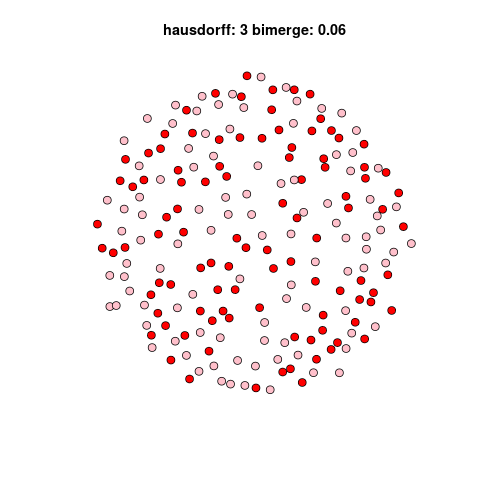
\includegraphics[scale=0.5]{images/AD6-AD6-100-IM.png}
  \caption{\(\Sigma_1 = \Sigma_2 = \braces{A, B, C, D}\)}
  \label{ad6ad6}
\end{minipage}
\begin{minipage}{0.45\textwidth}
\centering
  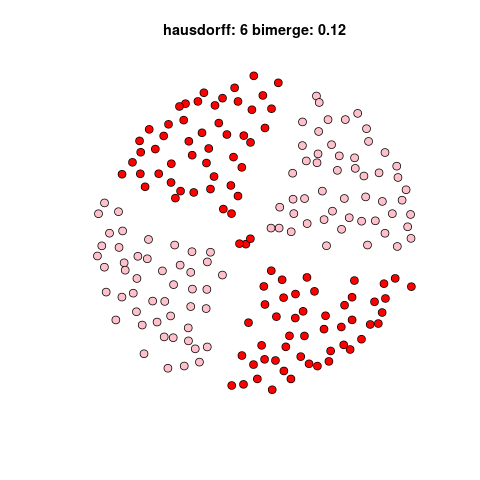
\includegraphics[scale=0.5]{images/AD6-DG6-100-IM.png}
  \caption{\(\Sigma_1 = \braces{A, B, C, D}\) and
            \(\Sigma_2 = \braces{D, E, F, G}\)}
  \label{ad6dg6}
\end{minipage}
\end{figure}

A numerical experiment was run
where \(100\) strings (\(A\)) of length \(6\) was
uniformly generated at random from alphabet \(\Sigma_1\),
and another \(100\) strings (\(B\)) of length (6) was uniformly generated
at random from alphabet \(\Sigma_2\).

In one round of the experiment as shown in Figure~\ref{ad6ad6},
we set \(\Sigma_1 = \Sigma_2 = \braces{A, B, C, D}\).
In other words,
the set \(A\) (dark red) and \(B\) (light red)
were generated from the same distribution.
The figure displayed is a force plot on a complete graph
(in this case \(K_{200}\))
where the edge weights are weighted by inverse edit distance.
That is, each dot (vertex) represents a string,
and dots that are visually closer to each other will tend to have higher
weights (and thus higher attractive force) due to a smaller edit distance.

The idea behind this type of plot is to see how well a metric is able to
correlate to our understanding of string similarity with respect to
the edit distance.
In the first round, because \(A\) and \(B\) were generated from the same
probability distribution, the force plot has a difficult time separating them,
and therefore yields a strong mixing.
The Hausdorff metric is \(3\), meaning that all strings in \(A\) and \(B\)
are at most edit distance \(3\) apart.
The bi-merge cost \(m\) is 0.06.

In the second round the experimental set up was the same and
the results are displayed in Figure~\ref{ad6dg6},
except now we have
\(\Sigma_1 = \braces{A, B, C, D}\) and
\(\Sigma_2 = \braces{D, E, F, G}\).
Again 100 strings of length \(6\) were generated
uniformly at random from \(\Sigma_1\) for \(A\)
and 100 strings of length \(6\) were generated
uniformly at random from \(\Sigma_2\) for \(B\).

We note that this time the Hausdorff distance between \(A\) and \(B\)
is \(6\),
which is expected because the alphabets from which they were uniformly
generated only shares \(D\) in common.
Likewise, the bi-merge cost is higher, now at \(0.12\).
Finally, because \(A\) and \(B\) are generated from fairly different
alphabets (which only share one letter),
the corresponding languages have strong visual separation,
which is desired.


In summary, although the bi-merge cost is not a metric,
the techniques employed here for visualizing the distance of two strings
appears to be useful,
can be utilized for similar problems.


